\section{Hash Table}
La Hash Table è una struttura di dati che memorizza i dati in modo associativo. In una tabella, i dati sono memorizzati in un formato array, dove ogni valore di dati ha un proprio valore di indice univoco. L'accesso ai dati diventa molto veloce se si conosce l'indice del dato desiderato.\\~\\
In questo modo, diventa una struttura di dati incui le operazioni di inserimento e ricerca sono molto veloci, indipendentemente dalla dimensione dei dati. La Hash Table utilizza un array come supporto di memorizzazione e usa la tecnica dell'Hash per generare un indice in cui un elemento deve essere inserito o da cui deve essere individuato. \\~\\
In particolare, si considera $U$ come insieme (universo) della chiavi, visto come $I = 0,1, \ldots,|U|-1$. La Hash Table $T$ viene vista come array $T[0,...|U|-1]$, in cui un elemento $x$ è inserito in $T[x.key]$.

\begin{center}
    \begin{tabular}{c}
        \\ 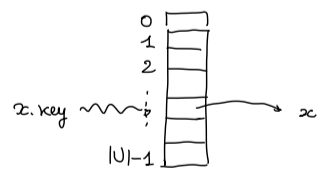
\includegraphics[width=0.4\textwidth]{image/HashTable.png} \\ \\
    \end{tabular}
\end{center}

\paragraph{Problemi:}
\begin{itemize}
    \item Non è possibile avere oggetti con la stessa chiave
    \item OK se il numero $|U|$ è piccolo
\end{itemize}

\begin{mdframed}
\begin{lstlisting}[mathescape=true]
INSERT(T,x)
1   T[x.key] = x        $\Theta(1)$
\end{lstlisting}
\end{mdframed}
\begin{mdframed}
\begin{lstlisting}[mathescape=true]
DELETE(T,x)
1   T[x.key] = NULL     $\Theta(1)$
\end{lstlisting}
\end{mdframed}
\begin{mdframed}
\begin{lstlisting}[mathescape=true]
SEARCH(k)
1   return T[k]         $\Theta(1)$
\end{lstlisting}
\end{mdframed}

\newpage
\subsection{Esempio}
\paragraph{Problema:} consideriamo che la key sia di 8 caratteri (8 bit per rappresentare un carattere). Risulta molto costosa in termini di memoria la tabella hash.
\paragraph{Obiettivo:} usare quantità di memoria proporzionale al numero di elementi da memorizzare.
\paragraph{Idea:} creazione di una tabella $T$ di dimensione $m << |U|$
\begin{equation*}
    h: U \rightarrow \{0, 1, \dots, m-1\}
\end{equation*}
Se $n>m \Rightarrow \exists\; x_1,x_2:h(x_1.key) = h(x_2.key) \Rightarrow$ conflitto \\~\\
Dove:
\begin{itemize}
    \item $n = $ \# elementi memorizzati nella tabella $T$
    \item $m = $ \# celle
\end{itemize}

La collisione verifica con $n = $ numero di elementi memorizzati se $m <<|U|$ se $n > m$. \\~\\

Il principio è il pigeonhole principle, quindi nella tabella hash, ogni valore trova una corrispondenza. 
Il pigeonhole principle è una delle idee più semplici ma più utili della matematica e può aiutarci in questo caso. 
Una versione di base dice che se ($N+1$) piccioni occupano $N$ buche, allora in qualche buca devono esserci almeno 2 piccioni. 
Quindi, se 5 piccioni occupano 4 buche, deve esserci una buca con almeno 2 piccioni.

\subsection{Chaining}
Il Chaining propone come soluzione quella di mettere sulla tabella liste dinamiche di elementi, invece che singoli elementi, in modo che in caso si incorra in una cella già occupata dopo un hashing, l'elemento venga inserito in coda (o in testa) alla lista. Nell'approccio di concatenamento, la tabella hash è una matrice di elenchi collegati, cioè ogni indice ha un proprio elenco collegato.Tutte le coppie chiave-valore mappate allo stesso indice saranno memorizzate nell'elenco collegato di quell'indice.

\begin{center}
    \begin{tabular}{c}
        \\ 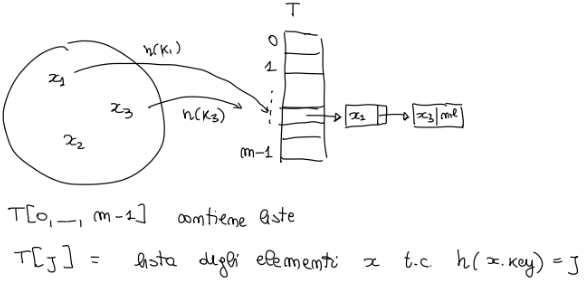
\includegraphics[width=0.7\textwidth]{image/Chaining.png} \\ \\
    \end{tabular}
\end{center}

\newpage
\begin{mdframed}
\begin{lstlisting}[mathescape=true]
INSERT(T,x)
1   T[x.key] = x           $\Theta(1)$
\end{lstlisting}
\end{mdframed}
\begin{mdframed}
\begin{lstlisting}[mathescape=true]
DELETE(T,x)
1   T[h(x.key)] = NULL     $\Theta(1)$
\end{lstlisting}
\end{mdframed}
\begin{mdframed}
\begin{lstlisting}[mathescape=true]
SEARCH(k)
1   return T[h(k)]         $\Theta(n)$
\end{lstlisting}
\end{mdframed}
L'operazione peggiore è quella di ricerca, dove alla peggio la complessità è lineare.

\subsection{Caso medio}
\paragraph{Partenza:}
\begin{itemize}
    \item $m =$ \# celle tabella
    \item $n =$ \# elementi inseriti
    \item $\alpha = \frac{n}{m}$ che può essere minore, maggiore oppure uguale ad 1
\end{itemize}

Ogni elemento $x$ in input ha la stessa probabilità di $\frac{1}{m}$ di essere "indirizzato" in una qualunque delle $m$ celle. Esso è indicato come $n_j =$ lunghezza lista in $T[j]$.

\begin{center}
    \begin{tabular}{c}
        \\ 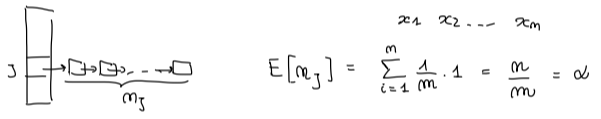
\includegraphics[width=0.7\textwidth]{image/ChainingCasoBase.png} \\ \\
    \end{tabular}
\end{center}

\paragraph{Costo medio di Search:} dato dalla ricerca di una chiave non presente $k$ \\~\\
$\begin{rcases}
    \begin{rcases}
        \text{calcolo } h(k) = j \\
        \text{accedo alla lista } T[j]
    \end{rcases}
    \Rightarrow O(1) \\
    \text{scorro la lista } T[j] \text{ fino in fondo } (n_j \text{elementi}) \Rightarrow n_j
\end{rcases} \Rightarrow \Theta(1 + \alpha)$

\paragraph{Ricerca di una chiave:} presente \\~\\
$\begin{rcases}
    \begin{rcases}
        \text{calcolo } h(k) = j \\
        \text{accedo alla lista } T[j]
    \end{rcases}
    \Rightarrow O(1) \\
    \text{scorro la lista } T[j] \text{ fino in a trovare l'elemento con chiave } k
\end{rcases} \Rightarrow 1+\frac{n_j}{2} \Rightarrow 1+\frac{\alpha}{2}$ \\~\\

Più precisamente: cerco $x$ con chiave $x.key = k$.

\newpage
\subsection{Funzioni di Hash}
Se le chiavi fossero numero reali $k \in [0,1) \Rightarrow h(k)=|mx|$ \\~\\
L'ipotesi di Hash uniforme semplice dipende dalle probabilità con cui vengono estratti gli elementi da inserire; probabilità che in genere non sono note. Le funzioni hash che descriveremo assumono che le chiavi siano degli interi non negativi.

\paragraph{Metodo della divisione:}\;\\~\\
$\begin{rcases}
    U = \{0, 1, \ldots, |U|-1\} \\
    h(k) \in \{0, 1, \ldots, m-1\} \\
\end{rcases} \Rightarrow h(k) = k \mod m$ \\~\\

La scelta di $m$ è critica:
\begin{itemize}
    \item $m = 2^p$
    \item $m = 2^p - 1$
\end{itemize}
$h(k) = h(k')$ se $k$ si ottiene "permutando" $k'$.

\paragraph{Metodo della moltiplicazione:}
\begin{itemize}
    \item se $x \in [0,1) \Rightarrow h(x) = |(mx)|$
    \item chiave $k \in 0,1,\ldots,|U|-1$
    \item dato $k$
    \begin{itemize}
        \item fisso costante $A \in (0,1) \quad (0<A<1)$
        \item $k * A = k * A \mod 1$
    \end{itemize}
    \item $h(k) = |(m(k*A\mod1))|$
    \item[] \paragraph{pro:}
    \begin{itemize}
        \item $m$ non critico
        \item $A$ non critico
    \end{itemize}
    \item[] \paragraph{contro:}
    \begin{itemize}
        \item $m = 2^p$
        \item $w =$ \# bit particolare
        \item $A = \frac{q}{2^w} \quad (0<q<2)$
        \item $m(k * A \mod 1) = m(k \frac{q}{2^w} \mod 1)$
    \end{itemize}
\end{itemize}

\newpage
\subsection{Open Addressing}
\paragraph{Idea:} memorizzo gli elementi dell'insieme dinamico solo nello spazio della tabella.
\begin{itemize}
    \item funzione di Hash $h(k,i)$
    \item $k$ chiave
    \item $i$ \# tentativo
\end{itemize}
La funzione Hash specifica l'ordine degli slot da sondare (provare) per una chiave (per inserire/ricercare/cancellare).
\begin{itemize}
    \item provo con $h(k,0)$
    \item se capito in una cella occupata, provo con $h(k,1)$
    \item poi con $h(k,2)$ e così via, fino a che non trovo una cella libera
    \item per esplorare tutta la tabella: $h(k,0), h(k,1), \dots, h(k,m-1) \quad \forall\; k \in U$
\end{itemize}

\paragraph{Operazioni possibili:}
\begin{mdframed}
\begin{lstlisting}[language=C]
INSERT(T,x)
1   i = 0
2   repeat
3       j = h(x.key,i)
4       if (T[j] = NULL) or (T[j] = DEL)
5           T[j] = x
6           return j
7       i = i + 1
8   until i = m
9   error
\end{lstlisting}
\end{mdframed}
\begin{mdframed}
\begin{lstlisting}[language=C]
SEARCH(T,k)
1   i = 0
2   repeat
3       j = h(k,i)
4       if T[j].key = k
5           return j
6       i = i + 1
7   until (i = m) or (T[j] = NULL)
8   return NOT FOUND
\end{lstlisting}
\end{mdframed}
\begin{mdframed}
\begin{lstlisting}[language=C]
DELETE(T,j)
1   T[j] = DEL
\end{lstlisting}
\end{mdframed}

L'Open Addressing risulta una soluzione inefficiente in caso avvengano molte cancellazioni. Similmente, giusto per citarla, è possibile anche attuare una randomizzazionedell'input, per avere una distribuzione più uniforme delle chiavi nelle liste e non dipendente dall'input. La complessità sarà sempre $\Theta(1+\alpha)$

\subsection{Hashing Uniforme}
Ogni elemento determina con la stessa probabilità una qualunque delle $m!$ sequenze di ispezione. \\~\\
In questo contesto le funzioni di Hash sono:
\begin{itemize}
    \item \textbf{Ispezione Lineare:} fisso $h(k)$ funzione di hash e $h'(k+1) = (h(k) + i) \mod m$
    \begin{itemize}
        \item vantaggi: semplice; poche permutazioni  ($m$ dipende solo da $h'(k)$)
        \item svantaggi: addensamento primario (addensamenti di celle occupate)
    \end{itemize}
    \item \textbf{Ispezione Quadratica:}
    \begin{itemize}
        \item dato $h(k)$ funzione di hash $h'(k,i) = (h(k) + c_1i + c_2i^2) \mod m$ con $c_1, c_2$ opportune e $c_2 > 0$
        \item addensamento secondario (addensamento quadratico di celle occupate)
        \item \# sequenze di ispezione dipende solo da$h(k) \mod m \Rightarrow m$ possibilità
    \end{itemize}
    \item \textbf{Doppio Hashing:} siano $h_1(k), h_2(k)$ funzioni di Hash di un solo argomento $\Rightarrow h(k,i) = (h_1(k) + ih_2(k) \mod m)$
\end{itemize}

\paragraph{Costo} \;\\~\\
Il costo della funzione \verb|Search| con hashing uniforme è riassunta come: $0 \leq \alpha = \frac{n}{m} \leq 1$
\begin{itemize}
    \item Ricerca di una chiave non presente:
    \begin{itemize}
        \item $\frac{1}{1-\alpha}$ \quad se $\alpha < 1$
        \item $m$ \quad se $\alpha = 1$
    \end{itemize}
    \item Ricerca di una chiave presente:
    \begin{itemize}
        \item $\frac{1}{\alpha} \log(\frac{1}{1-\alpha}) \quad \alpha<1$
        \item $1 + \log m \quad \alpha=1$
    \end{itemize}
\end{itemize}

\newpage
